\section{Radiative Transfer Calculations}
%========================================
\label{sec:rt}
\subsection{Methodology}
%-----------------------
Monochromatic radiative transfer calculations were done at the various tabulated ATMS SRF frequencies using MonoRTM \cite{Payne_2008,Clough_2005} and the ECMWF83 profile set \cite{Matricardi_ECMWF564,ECMWF_profile_set2}. The subsequent spectra were then convolved with the tabulated SRFs using a simple numerical integration routine.

The temperature and water vapour from the ECMWF83 set are shown in figure \ref{fig:ECMWF83.AtmProfile} to provide an indication of the range of inputs. We realise 83 profiles is a small sample and are looking at repeating the calculations for a larger (1000's of profiles) data set. 

\begin{figure}[htp]
  \centering
  \includegraphics[scale=1]{graphics/atmprofile/ECMWF83.AtmProfile.eps}
  \caption{The temperature and water vapour profiles from the ECMWF83 profile dataset used in the radiative transfer calculations.}
  \label{fig:ECMWF83.AtmProfile}
\end{figure}


\subsection{Results}
%-------------------
The results for the different digitised, or measured, SRFs are presented here as brightness temperature differences from the boxcar SRF result, that is,
\begin{equation}
  \Delta T_B = T_{B,Boxcar} - T_{B,Measured}
\end{equation}
The $\Delta T_B$ values are displayed as a function of $T_{B,Boxcar}$ as well as a histogram of the differences. Only the results for those channels for which we have either SDL or NGAS digistised SRFs will be discussed here. Results for all the channels are shown in Appendix \ref{app:dtb}. Since the reference for the brightness temperatures differences is the boxcar SRF, it should also be noted that these comparisons are intended to highlight the impact of the differences between the various digitised SRFs, not necessarily to indicate which is ``better''.

\subsubsection{Single passband channels: 1, 4, 5, amd 9}
%......................................................
The $\Delta T_B$ scatterplots for the single passband channels 1, 4, 5, and 9 are shown in figure \ref{fig:sp_digitised_dtbs_scatter}, and the corresponding histograms are shown in figure \ref{fig:sp_digitised_dtbs_hist}. In all cases the SDL and NGAS digitisations decreased the $\Delta T_B$ values, although to different degrees.

\begin{figure}[htp]
  \centering
  \begin{tabular}{c c}
    \textsf{\textbf{(a)} Channel 1} &
    \textsf{\textbf{(b)} Channel 4} \\
    \includegraphics[bb=82 289 312 493,clip,scale=1.0]{graphics/dtb/atms_npp.ch1.TbStats.eps} &
    \includegraphics[bb=82 289 312 493,clip,scale=1.0]{graphics/dtb/atms_npp.ch4.TbStats.eps} \\\\

    \textsf{\textbf{(c)} Channel 5} &
    \textsf{\textbf{(d)} Channel 9} \\
    \includegraphics[bb=82 289 312 493,clip,scale=1.0]{graphics/dtb/atms_npp.ch5.TbStats.eps} &
    \includegraphics[bb=82 289 312 493,clip,scale=1.0]{graphics/dtb/atms_npp.ch9.TbStats.eps}
  \end{tabular}
  % the hand-crafted legend
  \setlength{\unitlength}{1cm}
  \begin{picture}(2.0,1.25)(0.0,0.45)
    \thicklines
    \color{blue}
    \put(0.0,0.7 ){\line(1,0){1}}
    \put(1.1,0.55){\sffamily NGAS}
    \color{green}
    \put(0.0,1.2 ){\line(1,0){1}}
    \put(1.1,1.05){\sffamily SDL}
    \color{red}
    \put(0.0,1.7 ){\line(1,0){1}}
    \put(1.1,1.55){\sffamily Table 12}
  \end{picture}
  \caption{Scatterplots of the calculated brightness temperature differences, $\Delta T_B$, as a function of the boxcar SRF $T_{B,Boxcar}$ for the single passband SDL and NGAS digitised SRFs}
  \label{fig:sp_digitised_dtbs_scatter}
\end{figure}

\begin{figure}[htp]
  \centering
  \begin{tabular}{c c}
    \textsf{\textbf{(a)} Channel 1} &
    \textsf{\textbf{(b)} Channel 4} \\
    \includegraphics[bb=312 289 538 493,clip,scale=1.0]{graphics/dtb/atms_npp.ch1.TbStats.eps} &
    \includegraphics[bb=312 289 538 493,clip,scale=1.0]{graphics/dtb/atms_npp.ch4.TbStats.eps} \\\\

    \textsf{\textbf{(c)} Channel 5} &
    \textsf{\textbf{(d)} Channel 9} \\
    \includegraphics[bb=312 289 538 493,clip,scale=1.0]{graphics/dtb/atms_npp.ch5.TbStats.eps} &
    \includegraphics[bb=312 289 538 493,clip,scale=1.0]{graphics/dtb/atms_npp.ch9.TbStats.eps}
  \end{tabular}
  % the hand-crafted legend
  \setlength{\unitlength}{1cm}
  \begin{picture}(2.0,1.25)(0.0,0.45)
    \thicklines
    \color{blue}
    \put(0.0,0.7 ){\line(1,0){1}}
    \put(1.1,0.55){\sffamily NGAS}
    \color{green}
    \put(0.0,1.2 ){\line(1,0){1}}
    \put(1.1,1.05){\sffamily SDL}
    \color{red}
    \put(0.0,1.7 ){\line(1,0){1}}
    \put(1.1,1.55){\sffamily Table 12}
  \end{picture}
  \caption{Histograms of the calculated brightness temperature differences, $\Delta T_B$, for the single passband SDL and NGAS digitised SRFs.}
  \label{fig:sp_digitised_dtbs_hist}
\end{figure}

The most striking change is for channel 1 (figs.\ref{fig:sp_digitised_dtbs_scatter}(a) and \ref{fig:sp_digitised_dtbs_hist}(a)) where both the magnitude and spread of the differences decreased markedly with the SDL digitised SRF producing a result much closer to that of a the boxcar response with little dependence on $T_{B,Boxcar}$. For channels 4 and 5 we have NGAS digitised SRF data and, despite the SRF differences being quite profound, the $\Delta T_B$ differences (figs.\ref{fig:sp_digitised_dtbs_scatter}(b),(c) and \ref{fig:sp_digitised_dtbs_hist}(b),(c)) do not really reflect this (at least, compared with the result for channel 1). The channel 9 radiometric differences (figs.\ref{fig:sp_digitised_dtbs_scatter}(d) and \ref{fig:sp_digitised_dtbs_hist}(d)) do not change too much between the Table 12 and NGAS SRF results despite the large differences in the SRF shape.

To further determine the cause of the $\Delta T_B$ differences in these channels, spectra were generated for a single profile (tropical climatology) for the channel bandwidth. These spectra are shown in figure \ref{fig:ch1_4_5_9.spectra}. Comparison of figure \ref{fig:ch1_4_5_9.spectra} with the SRFs shown in figure \ref{fig:sp_digitised_srfs} do not yield any obvious cause. Specifically, for:
\begin{description}
  \item[Channel 1:] The shapes of the Table 12 and SDL SRFs are not \textit{that} dissimilar. Furthermore, the variation of brightness temperature across the channel bandwidth is very small, $\sim$0.05K. Looking closely at figure \ref{fig:sp_digitised_srfs}(a), the only SRF difference that could be construed to cause the brightness temperatures we see are the higher magnitudes of the SDL SRF on the low-frequency band edge at frequencies less than 23.70GHz.

  \item[Channel 4:] Here we have an almost opposite effect compared to channel 1 in that the Table 12 and NGAS SRFs are very different, but the brightness temperatures not so much. There is a 1K variation across the channel spectrum of figure \ref{fig:ch1_4_5_9.spectra}(b) and, somewhat similarly to channel 1, one could theorise that in this case the higher-frequency band edge of the NGAS SRF compensates for the much smaller in-band magnitudes.

  \item[Channel 5:] The results here mirror those of channel 4 but with larger magnitudes most likely due to the larger 4K variation across the channel spectrum of figure \ref{fig:ch1_4_5_9.spectra}(c).

  \item[Channel 9:] Here we see a much larger ($\sim$6K), but also very non-linear, variation across the channel spectrum of figure \ref{fig:ch1_4_5_9.spectra}(d). Given the results for the Table 12 and NGAS SRF data (fig.\ref{fig:sp_digitised_dtbs_scatter}(d)) do not change much given the large SRF differences (fig.\ref{fig:sp_digitised_srfs}(d)) viewing the in-band spectrum for a single profile does not yield too much insight.
\end{description}
 
\begin{figure}[htp]
  \centering
  \includegraphics[scale=1.0]{graphics/spectra/ch1_4_5_9.eps}
  \caption{Spectra generated using MonoRTM for tropical climatology for the NPP ATMS single passband channels for which there exists SDL and NGAS digitised SRFs.}
  \label{fig:ch1_4_5_9.spectra}
\end{figure}


\subsubsection{Quadruple passband channels: 12, 13, 14, and 15}
%..............................................................
The $\Delta T_B$ scatterplots for the quadruple passband channels 12, 13, 14, and 15 are shown in figure \ref{fig:qp_digitised_dtbs_scatter}, and the corresponding histograms are shown in figure \ref{fig:qp_digitised_dtbs_hist}.

\begin{figure}[htp]
  \centering
  \begin{tabular}{c c}
    \textsf{\textbf{(a)} Channel 12} &
    \textsf{\textbf{(b)} Channel 13} \\
    \includegraphics[bb=82 289 312 493,clip,scale=1.0]{graphics/dtb/atms_npp.ch12.TbStats.eps} &
    \includegraphics[bb=82 289 312 493,clip,scale=1.0]{graphics/dtb/atms_npp.ch13.TbStats.eps} \\\\

    \textsf{\textbf{(c)} Channel 14} &
    \textsf{\textbf{(d)} Channel 15} \\
    \includegraphics[bb=82 289 312 493,clip,scale=1.0]{graphics/dtb/atms_npp.ch14.TbStats.eps} &
    \includegraphics[bb=82 289 312 493,clip,scale=1.0]{graphics/dtb/atms_npp.ch15.TbStats.eps}
  \end{tabular}
  % the hand-crafted legend
  \setlength{\unitlength}{1cm}
  \begin{picture}(2.0,1.25)(0.0,0.45)
    \thicklines
    \color{blue}
    \put(0.0,0.7 ){\line(1,0){1}}
    \put(1.1,0.55){\sffamily NGAS}
    \color{green}
    \put(0.0,1.2 ){\line(1,0){1}}
    \put(1.1,1.05){\sffamily SDL}
    \color{red}
    \put(0.0,1.7 ){\line(1,0){1}}
    \put(1.1,1.55){\sffamily Table 12}
  \end{picture}
  \caption{Scatterplots of the calculated brightness temperature differences, $\Delta T_B$, as a function of the boxcar SRF $T_{B,Boxcar}$ for the quadruple passband SDL and NGAS digitised SRFs}
  \label{fig:qp_digitised_dtbs_scatter}
\end{figure}

\begin{figure}[htp]
  \centering
  \begin{tabular}{c c}
    \textsf{\textbf{(a)} Channel 12} &
    \textsf{\textbf{(b)} Channel 13} \\
    \includegraphics[bb=312 289 538 493,clip,scale=1.0]{graphics/dtb/atms_npp.ch12.TbStats.eps} &
    \includegraphics[bb=312 289 538 493,clip,scale=1.0]{graphics/dtb/atms_npp.ch13.TbStats.eps} \\\\

    \textsf{\textbf{(c)} Channel 14} &
    \textsf{\textbf{(d)} Channel 15} \\
    \includegraphics[bb=312 289 538 493,clip,scale=1.0]{graphics/dtb/atms_npp.ch14.TbStats.eps} &
    \includegraphics[bb=312 289 538 493,clip,scale=1.0]{graphics/dtb/atms_npp.ch15.TbStats.eps}
  \end{tabular}
  % the hand-crafted legend
  \setlength{\unitlength}{1cm}
  \begin{picture}(2.0,1.25)(0.0,0.45)
    \thicklines
    \color{blue}
    \put(0.0,0.7 ){\line(1,0){1}}
    \put(1.1,0.55){\sffamily NGAS}
    \color{green}
    \put(0.0,1.2 ){\line(1,0){1}}
    \put(1.1,1.05){\sffamily SDL}
    \color{red}
    \put(0.0,1.7 ){\line(1,0){1}}
    \put(1.1,1.55){\sffamily Table 12}
  \end{picture}
  \caption{Histograms of the calculated brightness temperature differences, $\Delta T_B$, for the quadruple passband SDL and NGAS digitised SRFs}
  \label{fig:qp_digitised_dtbs_hist}
\end{figure}

The results group themselves into two categories: channels where the newly digitised SRFs decrease the $\Delta T_B$ values and their spread (channels 13 and 14, figs.\ref{fig:qp_digitised_dtbs_scatter}(b),(c) and \ref{fig:qp_digitised_dtbs_hist}(b),(c)) and channels where the converse is true (channels 12 and 15, figs.\ref{fig:qp_digitised_dtbs_scatter}(a),(d) and \ref{fig:qp_digitised_dtbs_hist}(a),(d)).

For the channel 13 and 14 case where the $\Delta T_B$ values decrease, we have both SDL and NGAS SRF data (see figs. \ref{fig:qp_digitised_srfs}(b) and (c)) which agree quite well, as do their respective $\Delta T_B$ results\footnote{This would indicate the digitisation methodolgies employed are not contributing significantly to any differences}. The most obvious difference between the SDL/NGAS and Table 12 SRFs is that the for the former the relative magnitudes of the ``outer'' bands, \#1 and \#4, are about 10\% less than that for the ``inner'' bands, \#2 and \#3. This is not seen in the Table 12 SRF data.

For channels 12 and 15, where we only have SDL SRF data to compare (fig.\ref{fig:qp_digitised_srfs}(a) and (d)), the band relative magnitudes are fairly uniform but the impact of the SRF differences manifest themselves with a much larger bias and spread. Thus the SRF differences are obviously significant, but it's not immediately clear from comparisons of figures \ref{fig:qp_digitised_srfs} and \ref{fig:qp_digitised_dtbs_scatter} what feature of the SRF differences produces larger $\Delta T_B$ values.

As with the single passband channels, spectra were generated for a single profile (tropical climatology) for the channel bandwidths. These spectra are shown in figure \ref{fig:ch12_13_14_15.spectra} along with the a plot-spanning monochromatic spectrum for context. Even though the channel bandwidths and positions about the O\subscript{2} absorptions lines in question are different, the trend of the radiances across teh channel bands are similar -- e.g. the range of brightness temperature change across a band is about the same for all channels, $\sim$10K. Thus, figure \ref{fig:ch12_13_14_15.spectra} doesn't really help reveal why the different SRFs of figure \ref{fig:qp_digitised_srfs} produce the bipolar results seen in figures \ref{fig:qp_digitised_dtbs_scatter} and \ref{fig:qp_digitised_dtbs_hist}.

\begin{figure}[htp]
  \centering
  \includegraphics[scale=1.0]{graphics/spectra/ch12_13_14_15.eps}
  \caption{Spectra generated using MonoRTM for tropical climatology for the NPP ATMS quadruple passband channels for which there exists SDL and NGAS digitised SRFs. The portion of the spectrum  to which the channels are sensitive are represented by the heavy black lines. The full spectrum (magenta coloured line) is there for context.}
  \label{fig:ch12_13_14_15.spectra}
\end{figure}

